\documentclass[12pt,a4paper]{article}
\usepackage{amsthm}
\usepackage{amsmath} 
\usepackage[serbian]{babel}

\usepackage{graphicx}
\usepackage{float}

\usepackage{multicol}

\newtheorem{thm}{Teorema}[section]
\theoremstyle{definition}
\newtheorem{dfn}{Definicija}[section]
\theoremstyle{remark}
\newtheorem{no}{Napomena}[section]
\theoremstyle{plain}
\newtheorem{lem}[thm]{Lema}

% text width and height
\textwidth 16cm
\textheight 23cm

% distance from the top
\voffset -1.5cm

% distance from the left
\hoffset 0cm
\oddsidemargin 0mm

% distance from the bottom
\footskip 1.5cm

\linespread{1}

\setlength\parindent{0pt}

\usepackage{minted}

\title{Primena fazi logike u obradi slika}
\author{Jelena Mrdak, mi15021\\ Tijana Jevti\' c}

\begin{document}
\maketitle
\tableofcontents

\section{FCM}
\label{sec:FCM}
Fuzzy C-means (FCM) je jedan od najpopularnijih algoritama za fazi klasterovanje. U ovom poglavlju \' cemo ga najpre detaljno opisati, a zatim \' cemo ga iskoristiti za binarizaciju slike.\\

Cilj ovog algoritma je da skup $X=\{x_{1}, x_{2}, ..., x_{n}\}$ particioni\v se na $k$ delova (klastera) po 
nekom kriterijumu. Preciznije, kriterijum je minimizacija slede\' ce funkcije:
\begin{equation*}
 F(\bar{w}, \bar{c}) = \sum_{i=1}^{n}\sum_{j=1}^{k}w_{ij}^{m}\left\|x_{i}-c_{j}\right\|^{2},
\end{equation*}
gde $w_{ij}\in [0, 1]$ predstavlja pripadnost ta\v cke $x_{i}$ $j$-tom klasteru i $\sum_{j=1}^{k}w_{ij}=1$, dok je $c_{j}$ centroid $j$-tog klastera. Realni parametar $m>1$ predstavlja faktor fazifikacije i on se zadaje unapred.
U nastavku \' cemo preciznije odrediti ove koeficijente. Sada \' cemo samo ukratko opisati korake algoritma.\\

FCM je veoma sli\v can algoritmu k-means i sastoji se iz slede\' cih koraka:
\begin{itemize}
  \item Izabrati broj klastera $k$.
  \item Svakoj ta\v cki $x_{i}$ dodeliti koeficijente $w_{ij} \in [0, 1], j=1,2,..., k$.
  \item Ponavljati sve dok ne do\dj e do konvergencije:
    \begin{itemize}
      \item Izra\v cunati centroide za svaki klaster.
      \item A\v zurirati koeficijente.
    \end{itemize}
  \item Ta\v cku $x_{i}$ dodeliti klasteru kom najvi\v se pripada, tj. $r$-tom klasteru, gde je $w_{ir}=\max\limits_{j} w_{ij}$.
\end{itemize}

\begin{thm}
  Potrebni uslovi za minimizator $(\bar{w}^{*}, \bar{c}^{*})$ funkcije $F(\bar{w}, \bar{c})$ su:
  \begin{equation}\label{c}
    c_{j} = \frac{\sum\limits_{i=1}^{n} w_{ij}^m \cdot x_{i}}{\sum\limits_{i=1}^{n} w_{ij}^{m}}
  \end{equation}
  i
  \begin{equation}\label{w}
    w_{ij} = \frac{1}{\sum\limits_{u=1}^{k} \biggl(\frac{\left\|x_{i}-c_{j}\right\|}{\left\|x_{i}-c_{u}\right\|}\biggr)^{\frac{2}{m-1}}} 
  \end{equation}
\end{thm}
\begin{proof}
Prona\' ci \' cemo potencijalne ta\v cke lokalnih uslovnih ekstremuma. Koristi\' cemo Lagran\v zeve mno\v zioce. Posmatra\' cemo pomo\' cnu funkciju:
\begin{equation*}
  J(\bar{w}, \bar{c}, \bar{\lambda}) = \sum_{i=1}^{n}\sum_{j=1}^{k}w_{ij}^{m}\left\|x_{i}-c_{j}\right\|^{2} - \sum_{i=1}^{n}\lambda_{i}\biggl(\sum_{j=1}^{k}w_{ij}-1\biggr).
\end{equation*}

Ta\v cke koje tra\v zimo moraju da zadovoljavaju uslov $\nabla J=\textbf{0}$. Dakle,
  \begin{equation}\label{der_c}
  \frac{\partial J}{\partial c_{j}} = 0, 1\leq j \leq k
\end{equation}
  \begin{equation}\label{der_w}
  \frac{\partial J}{\partial w_{ij}} = 0, 1\leq i \leq n, 1\leq j \leq k 
\end{equation}
\begin{equation}\label{der_l}
  \frac{\partial J}{\partial \lambda_{i}} = 0, 1\leq i \leq n 
\end{equation}

  Re\v savanjem (\ref{der_c}) dobijamo (\ref{c}). Iz (\ref{der_w}) imamo
\begin{equation*}
  mw_{ij}^{m-1}\left\|x_{i}-c_{j}\right\|^{2} - \lambda_{i} = 0,
\end{equation*}
odnosno
\begin{equation}\label{wij}
  w_{ij} = \biggl(\frac{\lambda_{i}}{m\left\|x_{i}-c_{j}\right\|^{2}}\biggr)^{\frac{1}{m-1}}.
\end{equation}

Iz (\ref{der_l}) dobijamo:
\begin{align*}
  1&=\sum_{u=1}^{k}w_{iu}\\
   &=\sum_{u=1}^{k}\biggl(\frac{\lambda_{i}}{m\left\|x_{i}-c_{u}\right\|^{2}}\biggr)^{\frac{1}{m-1}}\\
   &=\sum_{u=1}^{k}\biggl(\frac{m\left\|x_{i}-c_{u}\right\|^{2}}{\lambda_{i}}\biggr)^{\frac{1}{1-m}}\\
   &=\sum_{u=1}^{k}\frac{(m\left\|x_{i}-c_{u}\right\|^{2})^{\frac{1}{1-m}}}{\lambda_{i}^{\frac{1}{1-m}}}\\
   &=\frac{1}{\lambda_{i}^{\frac{1}{1-m}}}\sum_{u=1}^{k}(m\left\|x_{i}-c_{u}\right\|^{2})^{\frac{1}{1-m}},
\end{align*}
pa zaklju\v cujemo da je
\begin{equation*}
  \lambda_{i} = \biggl(\sum_{u=1}^{k}(m\left\|x_{i}-c_{u}\right\|^{2})^{\frac{1}{1-m}}\biggr)^{1-m}.
\end{equation*}

Kona\v cno, zamenjuju\' ci poslednju jednakost u (\ref{wij}), dobijamo (\ref{w}). 
\end{proof}

FCM algoritam za odre\dj ivanje minimizatora funkcije $F$ je iteracija kroz potrebne uslove.

\subsection{Binarizacija slike}
\label{sec:binarizacija}
Ispod je prikazan kod za binarizaciju slike koji koristi FCM algoritam. Napominjemo da se zbog \v citljivosti koda u ovom delu nismo odlu\v cili za efikasnu implementaciju. O tome \' ce biti vi\v se re\v ci u narednoj sekciji.

\inputminted[tabsize=2,breaklines]{cpp}{codes/binarization.cpp}

Rezultat izvr\v savanja algoritma je prikazan ispod.
\begin{multicols}{2}
% first column
\begin{figure}[H]
\centering

\includegraphics[width=5cm]{images/storm_trooper.jpg}
  \caption{input}\label{storm_trooper_input}
\end{figure}
\columnbreak
% second column
\begin{figure}[H]
\centering
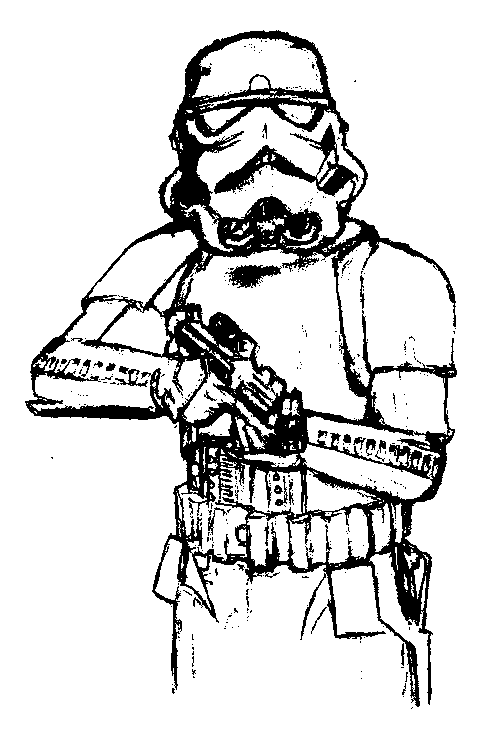
\includegraphics[width=5cm]{images/storm_trooper_binarized_fcm.png}
  \caption{output}
\end{figure}
\end{multicols}

\begin{multicols}{2}
% first column
\begin{figure}[H]
\centering
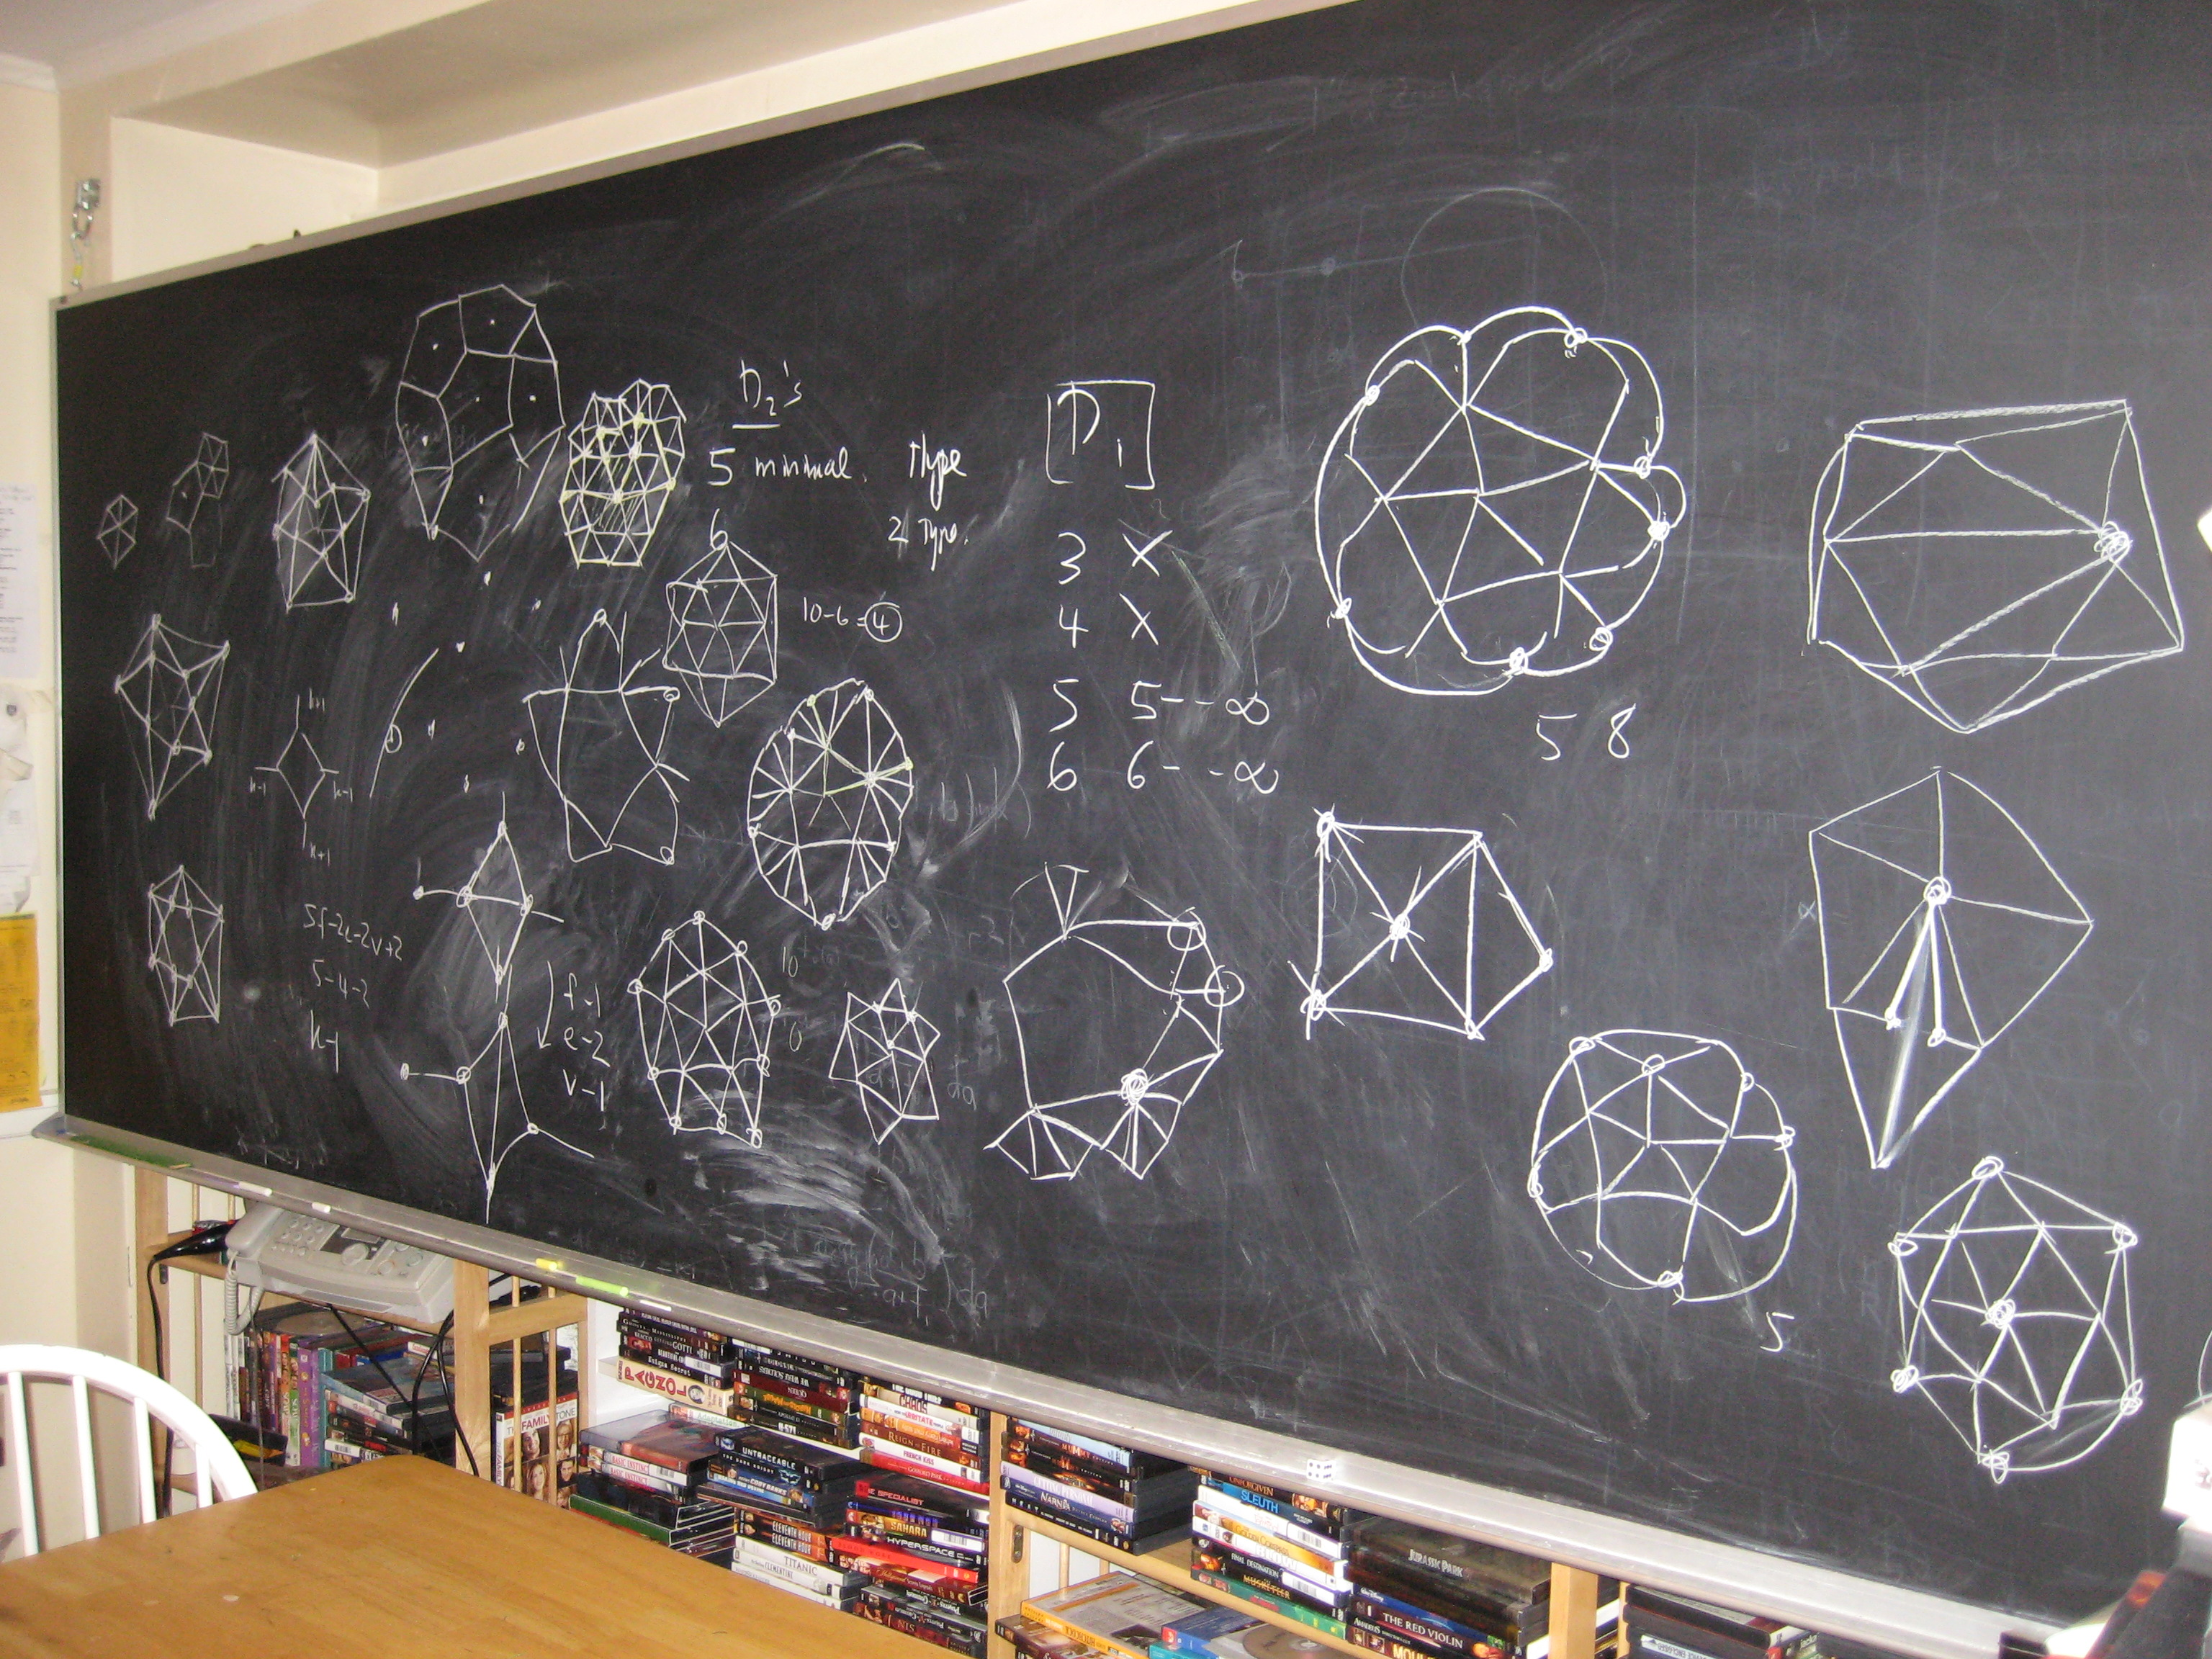
\includegraphics[width=7cm]{images/blackboard.jpg}
  \caption{input}\label{blackboard_input}
\end{figure}
\columnbreak
% second column
\begin{figure}[H]
\centering
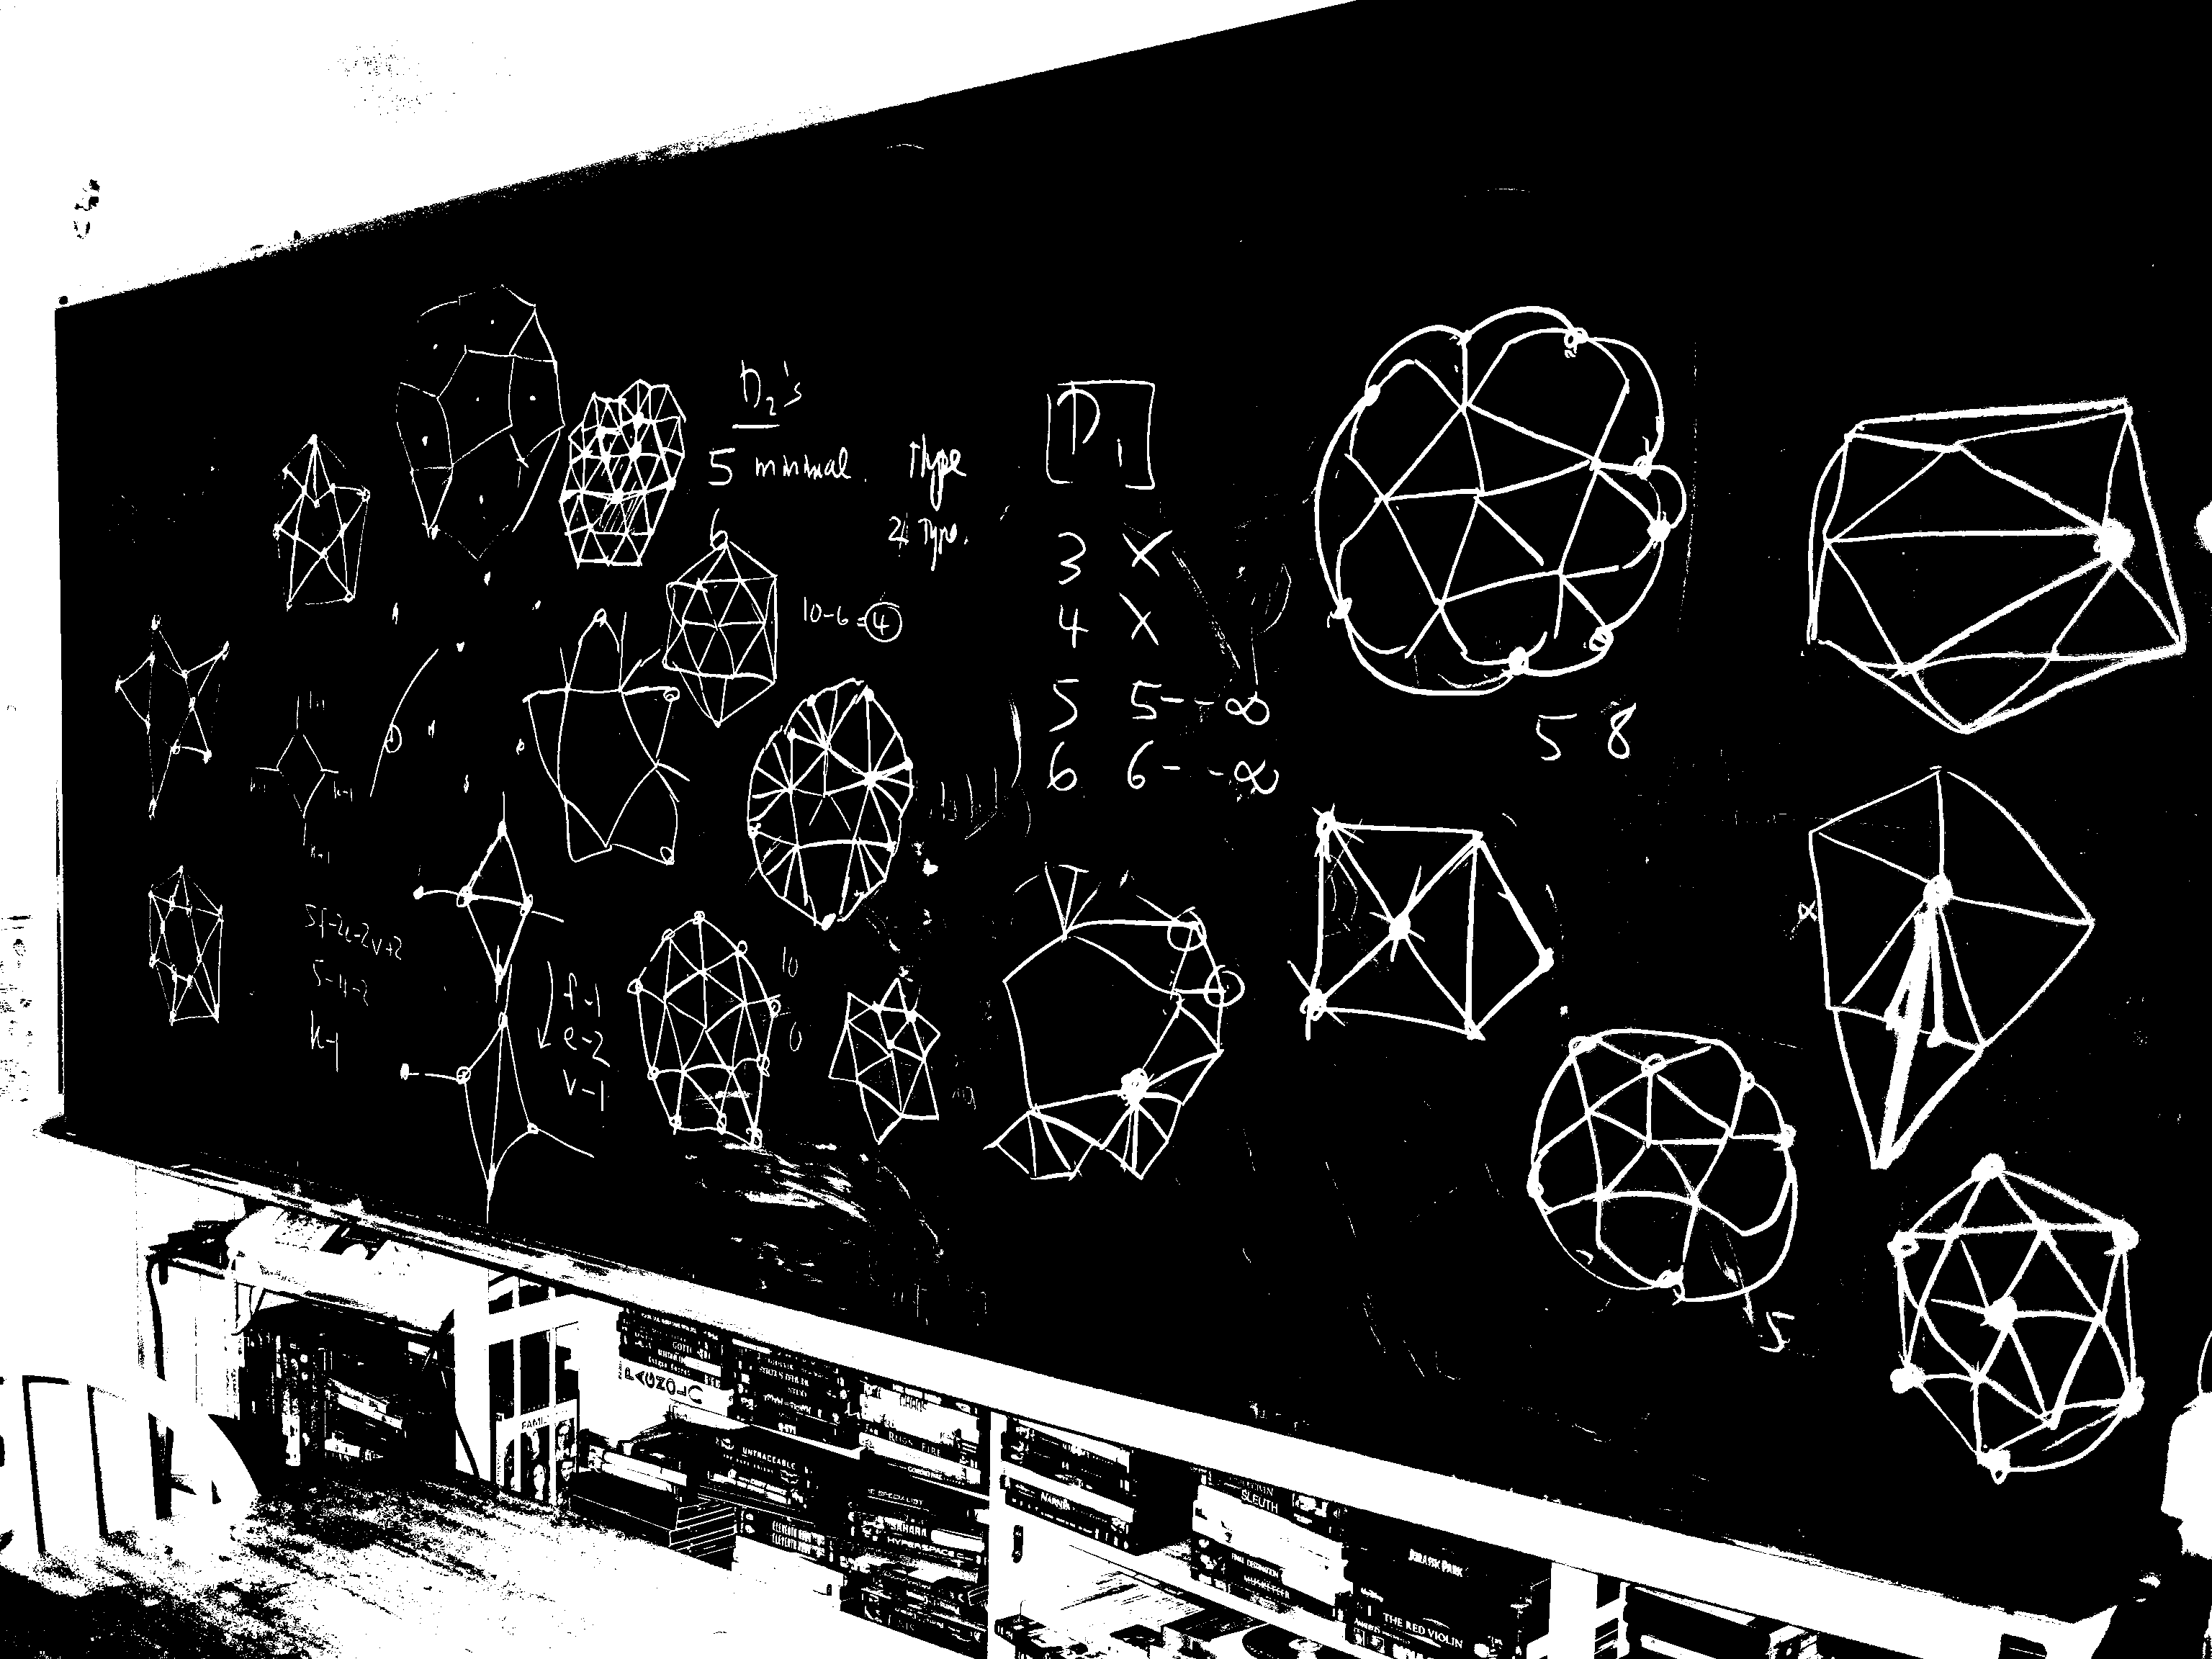
\includegraphics[width=7cm]{images/blackboard_binarized_fcm.png}
  \caption{output}
\end{figure}
\end{multicols}

\subsection{FCM i k-means}
U ovom odeljku \' cemo uporediti rezultate algoritama FCM i k-means, kao i vremena njihovih izvr\v savanja.

\begin{no}
  Koristi\' cemo efikasniju implementaciju FCM algoritma od one date u sekciji \ref{sec:binarizacija}.
\end{no}

Na slede\' cim slikama su prikazani rezultati.

\begin{multicols}{2}
% first column
\begin{figure}[H]
\centering
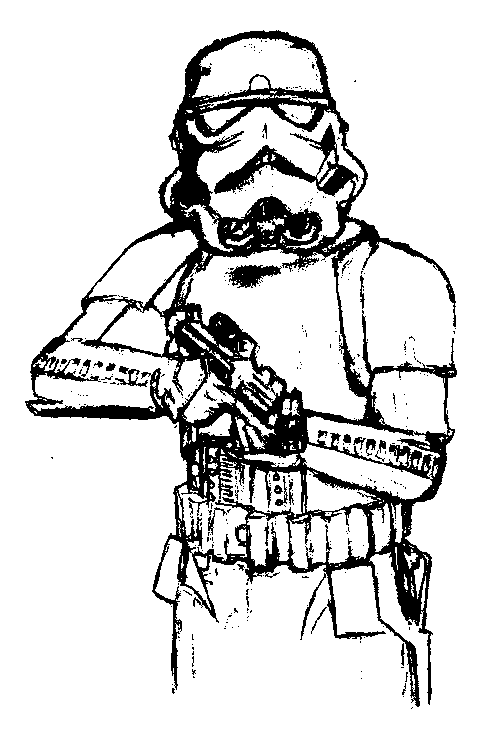
\includegraphics[width=5cm]{images/storm_trooper_binarized_fcm.png}
  \caption{FCM output}\label{storm_trooper_fcm}
 Broj iteracija: 7
\end{figure}
\columnbreak
% second column
\begin{figure}[H]
\centering
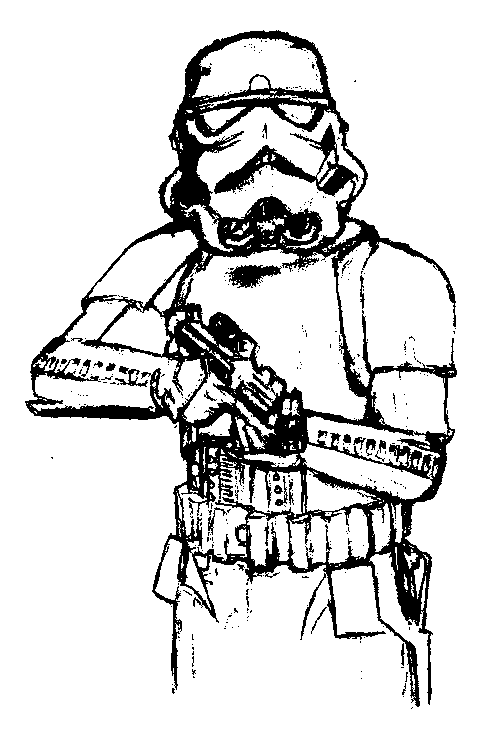
\includegraphics[width=5cm]{images/storm_trooper_binarized_kmeans.png}
  \caption{k-means output}\label{storm_trooper_kmeans}
 Broj iteracija: 6
\end{figure}
\end{multicols}

\newpage

\begin{multicols}{2}
% first column
\begin{figure}[H]
\centering
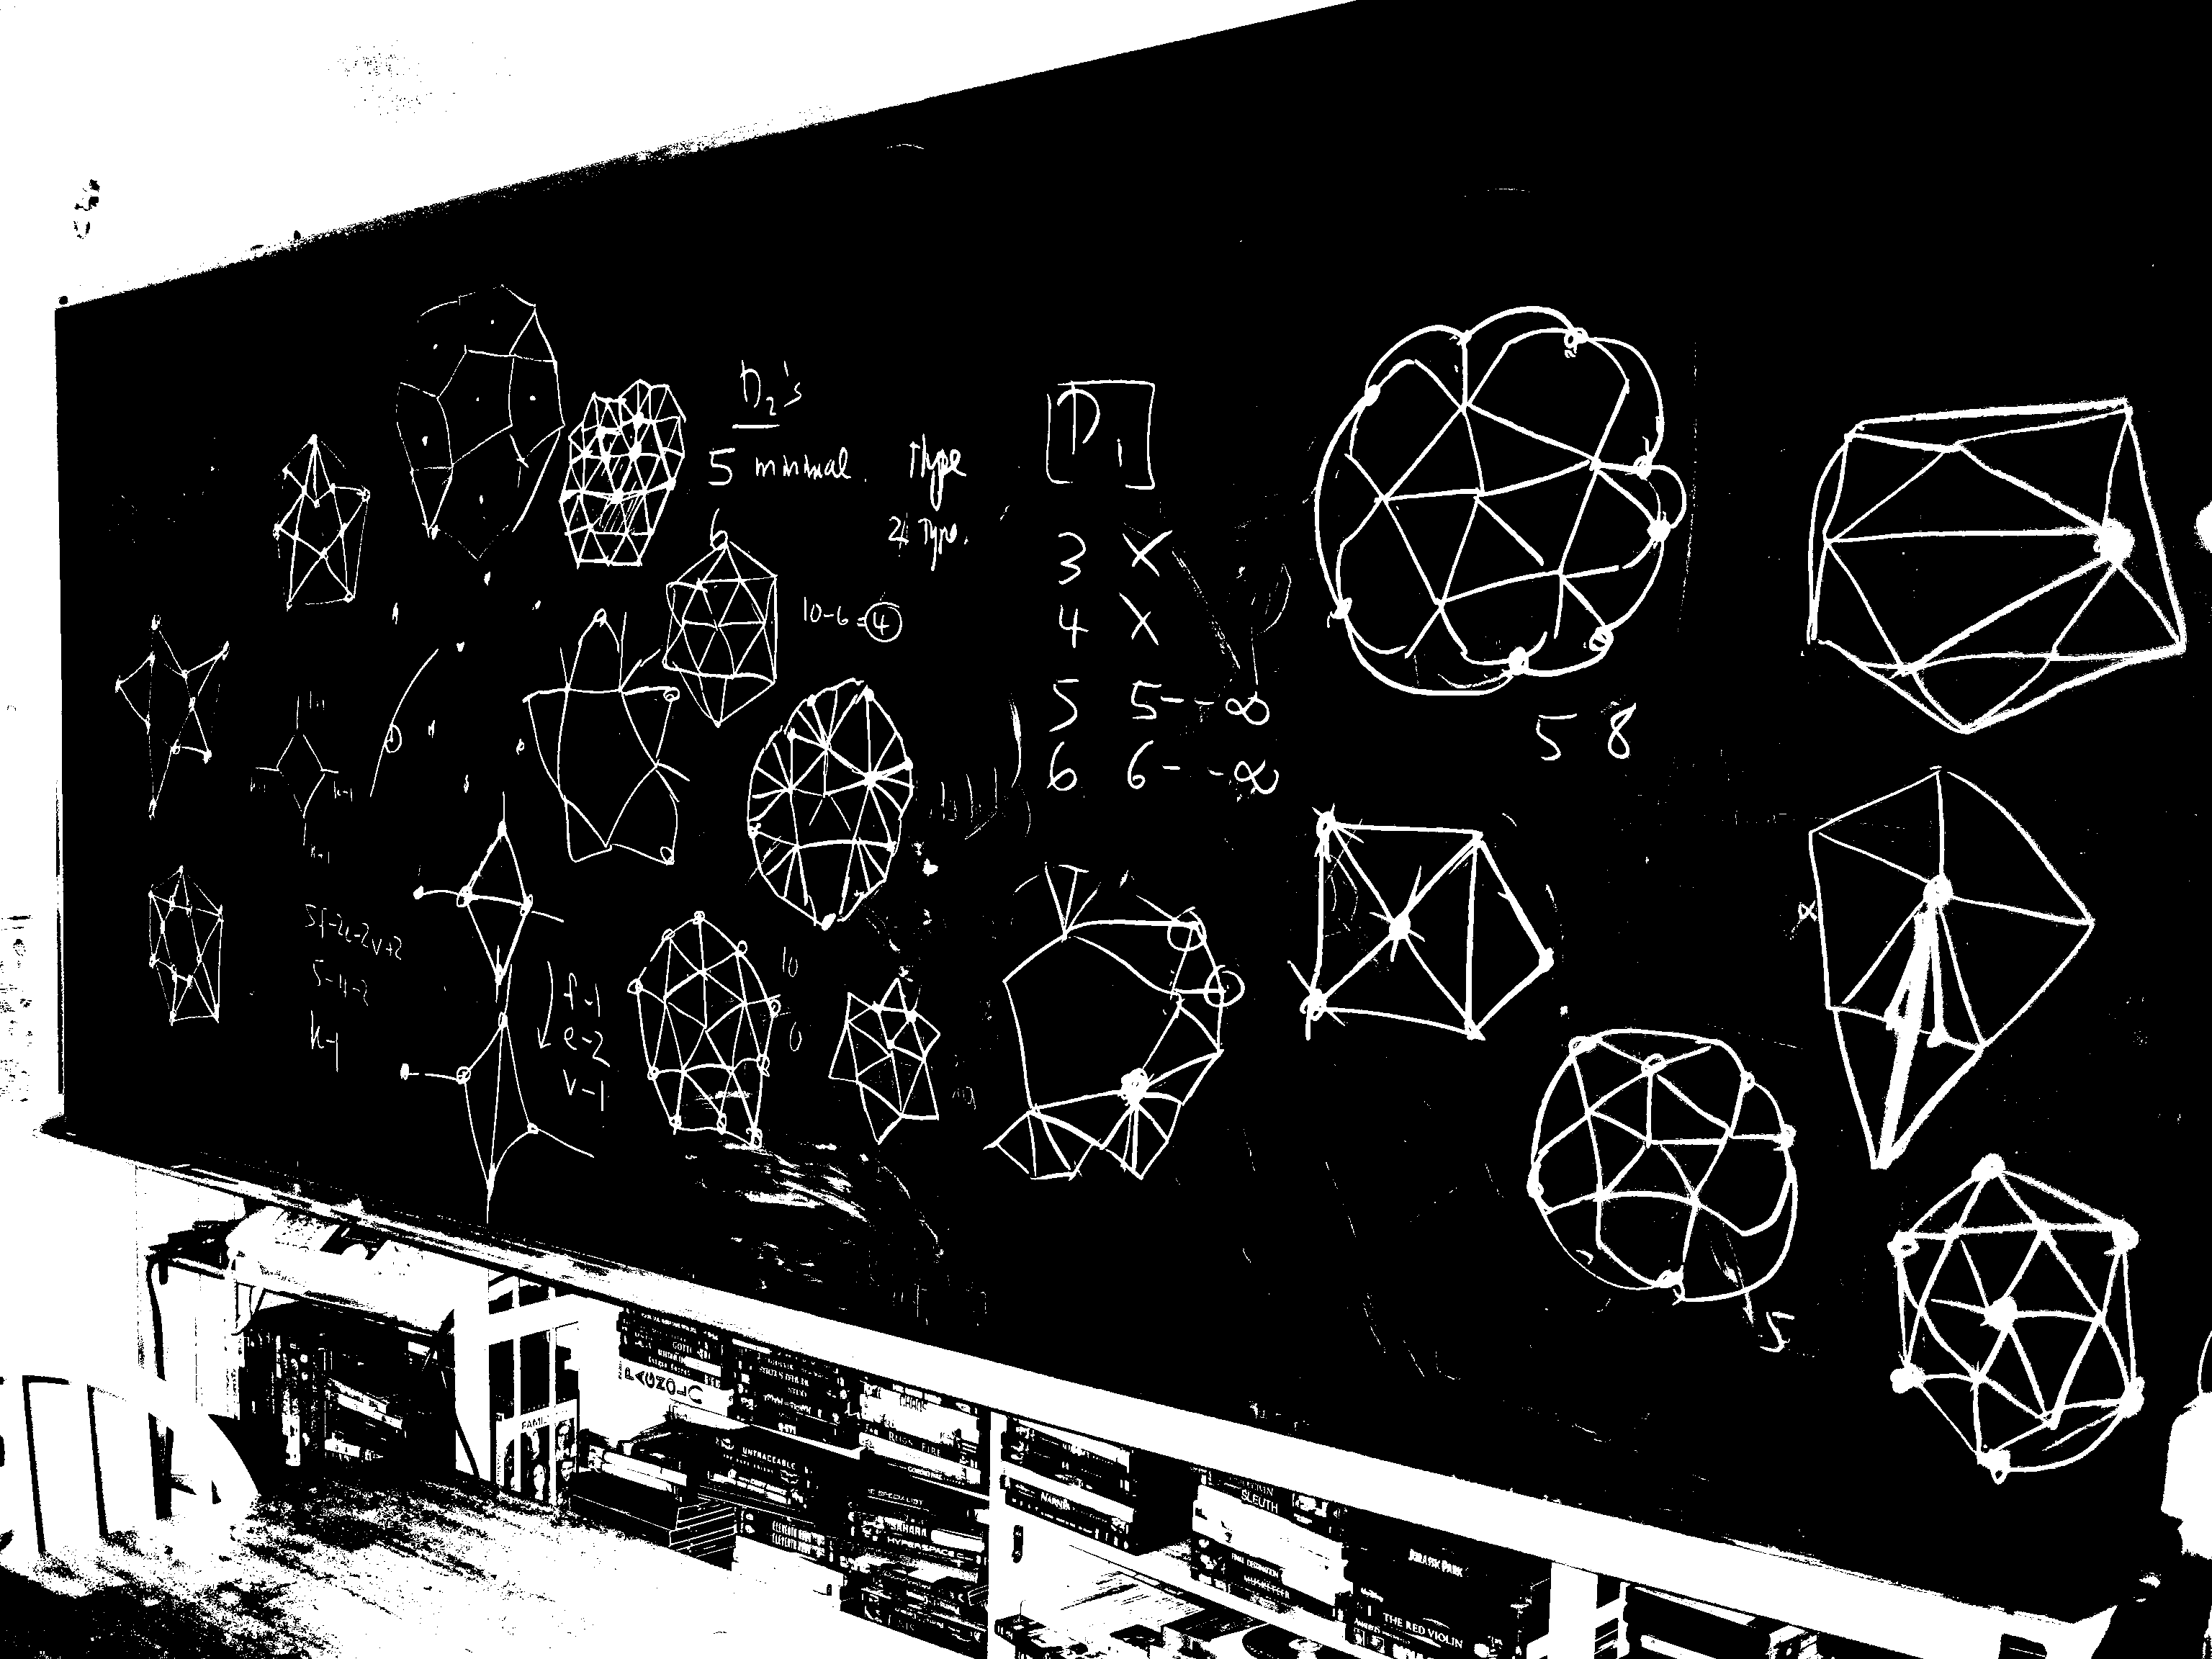
\includegraphics[width=7cm]{images/blackboard_binarized_fcm.png}
  \caption{FCM output}\label{blackboard_fcm}
 Broj iteracija: 7
\end{figure}
\columnbreak
% second column
\begin{figure}[H]
\centering
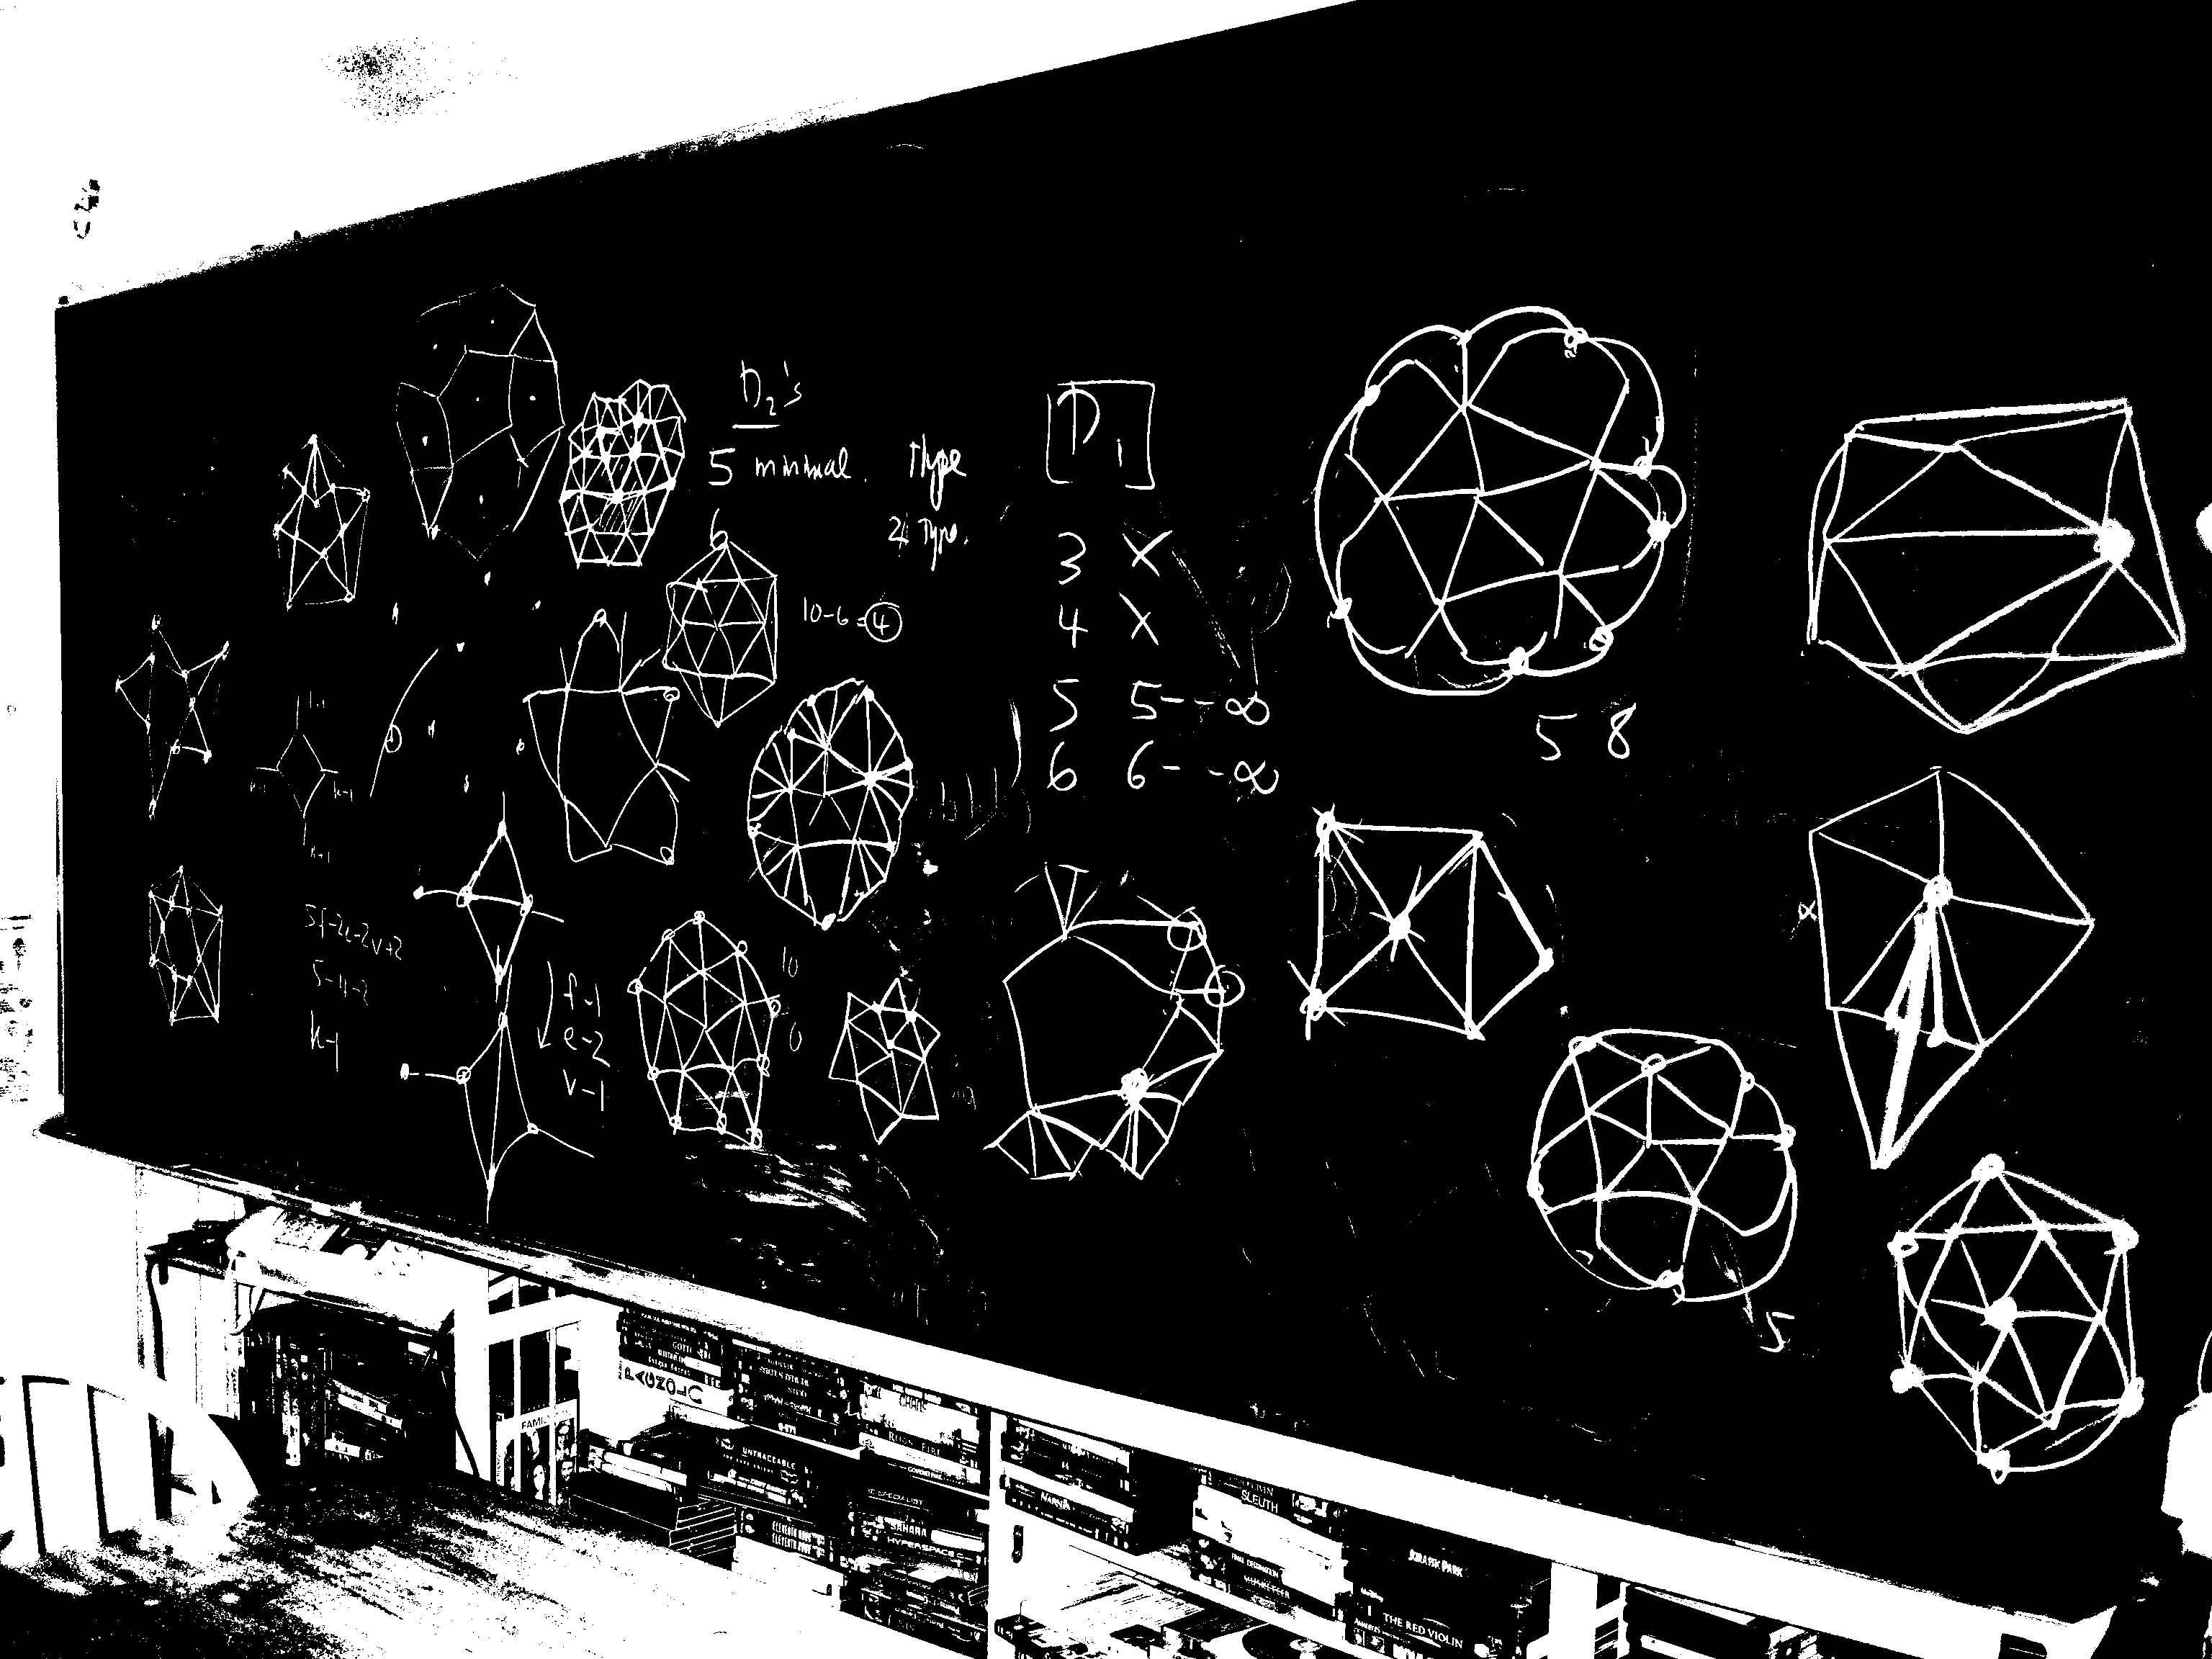
\includegraphics[width=7cm]{images/blackboard_binarized_kmeans.png}
  \caption{k-means output}\label{blackboard_kmeans}
  Broj iteracija: 7
\end{figure}
\end{multicols}

Mo\v zemo primetiti da su slike \ref{storm_trooper_fcm} i \ref{storm_trooper_kmeans} identi\v cne, dok se slike \ref{blackboard_fcm} i \ref{blackboard_kmeans} neznatno razlikuju. Me\dj utim, vremena izvr\v savanja se primetno razlikuju. U Tabeli \ref{vreme_storm} su prikazana vremena (u sekundama) potrebna da algoritmi obrade Sliku \ref{storm_trooper_input} 500, 1000 i 1500 puta. Sli\v cno, u Tabeli \ref{vreme_blackboard} su prikazana vremena potrebna da se obradi Slika \ref{blackboard_input} 50, 100 i 150 puta.

\begin{multicols}{2}
% first column
\begin{table}[H]
\centering
  \begin{tabular}{c|c|c}
  broj izvr\v savanja & FCM & k-means\\
  \hline
  500 & 4 & 21\\
  1000 & 8 & 42\\
  1500 & 12 & 63 
\end{tabular}
  \caption{Input Slika \ref{storm_trooper_input}}
  \label{vreme_storm}
\end{table}

\columnbreak

\begin{table}[H]
\centering
% second column
\begin{tabular}{c|c|c}
  broj izvr\v savanja & FCM & k-means\\
  \hline
  50 & 8 & 44\\
  100 & 17 & 89\\
  150 & 25 & 133 
\end{tabular}
  \caption{Input Slika \ref{blackboard_input}}
  \label{vreme_blackboard}
\end{table}
\end{multicols}

\end{document}
